\documentclass[12pt,a4paper]{article}

\usepackage[utf8]{inputenc}
\usepackage[margin=1in]{geometry}
\usepackage{graphicx}
\usepackage{hyperref}
\usepackage{listings}
\usepackage{xcolor}
\usepackage{float}
\usepackage{caption}
\usepackage{tikz}
\usetikzlibrary{shapes.geometric, arrows, positioning}

% Set styles for code blocks
\definecolor{codegreen}{rgb}{0,0.6,0}
\definecolor{codegray}{rgb}{0.5,0.5,0.5}
\definecolor{codepurple}{rgb}{0.58,0,0.82}
\definecolor{backcolour}{rgb}{0.95,0.95,0.92}

\lstdefinestyle{mystyle}{
    backgroundcolor=\color{backcolour},   
    commentstyle=\color{codegreen},
    keywordstyle=\color{magenta},
    numberstyle=\tiny\color{codegray},
    stringstyle=\color{codepurple},
    basicstyle=\ttfamily\footnotesize,
    breakatwhitespace=false,         
    breaklines=true,                 
    captionpos=b,                    
    keepspaces=true,                 
    numbers=left,                    
    numbersep=5pt,                  
    showspaces=false,                
    showstringspaces=false,
    showtabs=false,                  
    tabsize=2
}

\lstset{style=mystyle}

\title{Scientific Calculator Application: A DevOps CI/CD Pipeline Report}
\author{Shreyas Gangurde (MT2025117)}
\date{\today}

\begin{document}

\maketitle
\tableofcontents
\newpage

\section{Introduction}

This report documents the Continuous Integration and Continuous Deployment (CI/CD) pipeline built for a Command-Line Interface (CLI) Scientific Calculator written in C++. The core focus of this project is automating the complete lifecycle from code compilation to web-based deployment.

The pipeline automates:
\begin{itemize}
    \item Source code compilation utilizing CMake.
    \item Rigorous Unit and Integration Testing.
    \item Containerization of the application via Docker.
    \item Automated deployment to a server using Ansible.
    \item Serving the interactive C++ terminal application natively over a web browser via Gotty.
\end{itemize}

\section{DevOps Automation Workflow}
The following architecture visually tracks the flow of code from the developer's laptop to our live server environment.

\begin{figure}[H]
    \centering
    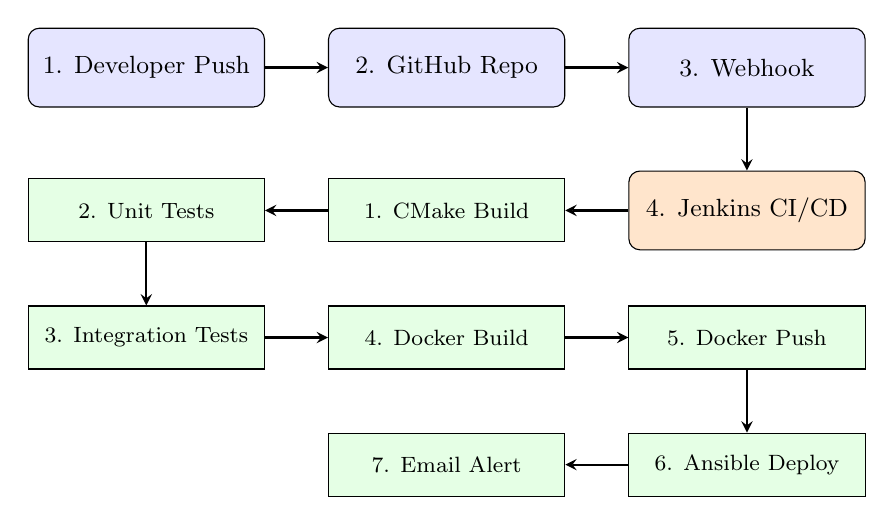
\begin{tikzpicture}[
        node distance=0.8cm and 0.8cm,
        box/.style={rectangle, draw, rounded corners, fill=blue!10, minimum width=3cm, minimum height=1cm, text centered, font=\small},
        stage/.style={rectangle, draw, fill=green!10, minimum width=3cm, minimum height=0.8cm, text centered, font=\footnotesize},
        arrow/.style={thick, ->, >=stealth}
        ]
        
        % Top Row: Dev to Webhook
        \node (dev) [box] {1. Developer Push};
        \node (github) [box, right=of dev] {2. GitHub Repo};
        \node (webhook) [box, right=of github] {3. Webhook};
        
        \draw [arrow] (dev) -- (github);
        \draw [arrow] (github) -- (webhook);
        
        % Middle Row: Jenkins
        \node (jenkins) [box, fill=orange!20, below=of webhook] {4. Jenkins CI/CD};
        \draw [arrow] (webhook) -- (jenkins);
        
        % Jenkins Pipeline First Row (Right to Left)
        \node (s1) [stage, left=of jenkins] {1. CMake Build};
        \node (s2) [stage, left=of s1] {2. Unit Tests};
        
        \draw [arrow] (jenkins) -- (s1);
        \draw [arrow] (s1) -- (s2);
        
        % Jenkins Pipeline Second Row (Left to Right)
        \node (s3) [stage, below=of s2] {3. Integration Tests};
        \node (s4) [stage, right=of s3] {4. Docker Build};
        \node (s5) [stage, right=of s4] {5. Docker Push};
        
        \draw [arrow] (s2) -- (s3);
        \draw [arrow] (s3) -- (s4);
        \draw [arrow] (s4) -- (s5);
        
        % Jenkins Pipeline Third Row (Right to Left)
        \node (s6) [stage, below=of s5] {6. Ansible Deploy};
        \node (s7) [stage, left=of s6] {7. Email Alert};
        
        \draw [arrow] (s5) -- (s6);
        \draw [arrow] (s6) -- (s7);
        
    \end{tikzpicture}
    \caption{DevOps Automation Workflow and Jenkins Pipeline Architecture mapping code from branch check-in to automated remote deployment.}
\end{figure}

\section{Jenkins Pipeline Architecture (\texttt{Jenkinsfile} Explanation)}

The backbone of this automated process is a declarative Jenkins Pipeline. Initially, this project was started as a Freestyle project in Jenkins to serve as a Proof of Concept (PoC). Once the core deployment and testing concepts were validated, the CI/CD structure was migrated to a robust declarative Pipeline to manage the complex, multi-stage lifecycle. The older Freestyle builds and the newer Pipeline builds have been appropriately renamed in the Jenkins dashboard to clearly signify their purpose.

Below is a detailed breakdown of each stage executed sequentially whenever new code is merged into the development branch.

\subsection{Stage 1: Build (CMake)}
This stage is responsible for generating the Makefiles and compiling the C++ source code into an executable binary.

\begin{lstlisting}[language=bash]
mkdir -p build && cd build
cmake ..
make
\end{lstlisting}
\textbf{Explanation:} We create an isolated \texttt{build} directory. \texttt{cmake ..} reads the root \texttt{CMakeLists.txt} to locate source files and external dependencies (like Google Test). \texttt{make} compiles the actual \texttt{./calculator} binary alongside the testing executables.

\subsection{Stage 2: Unit Tests}
This stage isolates and validates the core mathematical logic directly.

\begin{lstlisting}[language=bash]
cd build
ctest --output-on-failure -E "^IntegrationTest$"
\end{lstlisting}
\textbf{Explanation:} Using CTest (the test driver program for CMake), Jenkins triggers the isolated Google Test suite (\texttt{test\_calculator.cpp}). This rigorously checks fundamental operations like square roots of negative numbers, factorial constraints, and natural logarithms without invoking the User Interface layer. 

\subsection{Stage 3: Integration Tests}
This stage validates the interactive `ncurses` terminal interface exactly as a user would experience it.

\begin{lstlisting}[language=bash]
export TERM=xterm-256color
ctest --output-on-failure -R "^IntegrationTest$"
\end{lstlisting}
\textbf{Explanation:} Because the application actively reads keyboard arrows, we use the \texttt{expect} automation tool. We explicitly set the \texttt{TERM} environment variable so the CI server behaves like a real terminal. The Expect scripts mock pressing keyboard keys to navigate the calculator's menu and input numbers, asserting that the correct mathematical answers print directly to the screen.


\subsection{Stage 4: Build Docker Image}
Instead of deploying raw binaries, the application is packaged into a standardized container.

\begin{lstlisting}[language=bash]
DOCKER_BUILDKIT=1 docker build -t shreyasg28/sci-calc .
\end{lstlisting}
\textbf{Explanation:} Jenkins builds the \texttt{Dockerfile}. To drastically speed up consecutive builds, we utilize \textbf{Docker BuildKit} and specify \texttt{--mount=type=cache} layers for both \texttt{apt-get} package installations and \texttt{CMake} build objects. This ensures that unchanged dependencies are instantly reused rather than re-downloaded during every pipeline run. 

Crucially, this Dockerfile packages both our compiled calculator and a utility named \textbf{Gotty}. Gotty captures the backend Linux terminal process and serves it over HTTP WebSockets, entirely removing the need for end-users to use SSH to access the CLI application.

\subsection{Stage 5: Push Docker Image}
\begin{lstlisting}[language=bash]
docker push shreyasg28/sci-calc:latest
\end{lstlisting}
\textbf{Explanation:} Jenkins authenticates and pushes the successfully tested immutable container image globally to the Docker Hub registry for reliable distribution.

\subsection{Stage 6: Deploy (Ansible)}
\begin{lstlisting}[language=bash]
ansible-playbook -i ansible/inventory.ini ansible/deploy.yml --connection=local
\end{lstlisting}
\textbf{Explanation:} The final stage executes an Ansible playbook to manage the target server state. Ansible gracefully stops and removes any older running versions of the calculator, pulls the fresh image from Docker Hub, and spins up the new web-accessible container mapping host port 8081.

\subsection{Post-Build Actions}
Regardless of pipeline success or failure, a declarative post-action attempts to dispatch an email notification directly to the developer referencing the current build status and console log URL.

\begin{figure}[H]
    \centering
    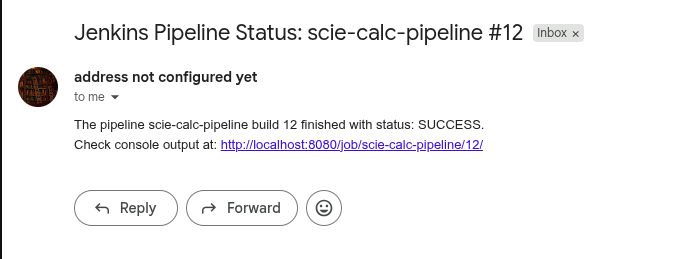
\includegraphics[width=0.9\textwidth]{images/email-notification.png}
    \caption{Email Notification dispatched by Jenkins indicating build result.}
\end{figure}

\begin{figure}[H]
    \centering
    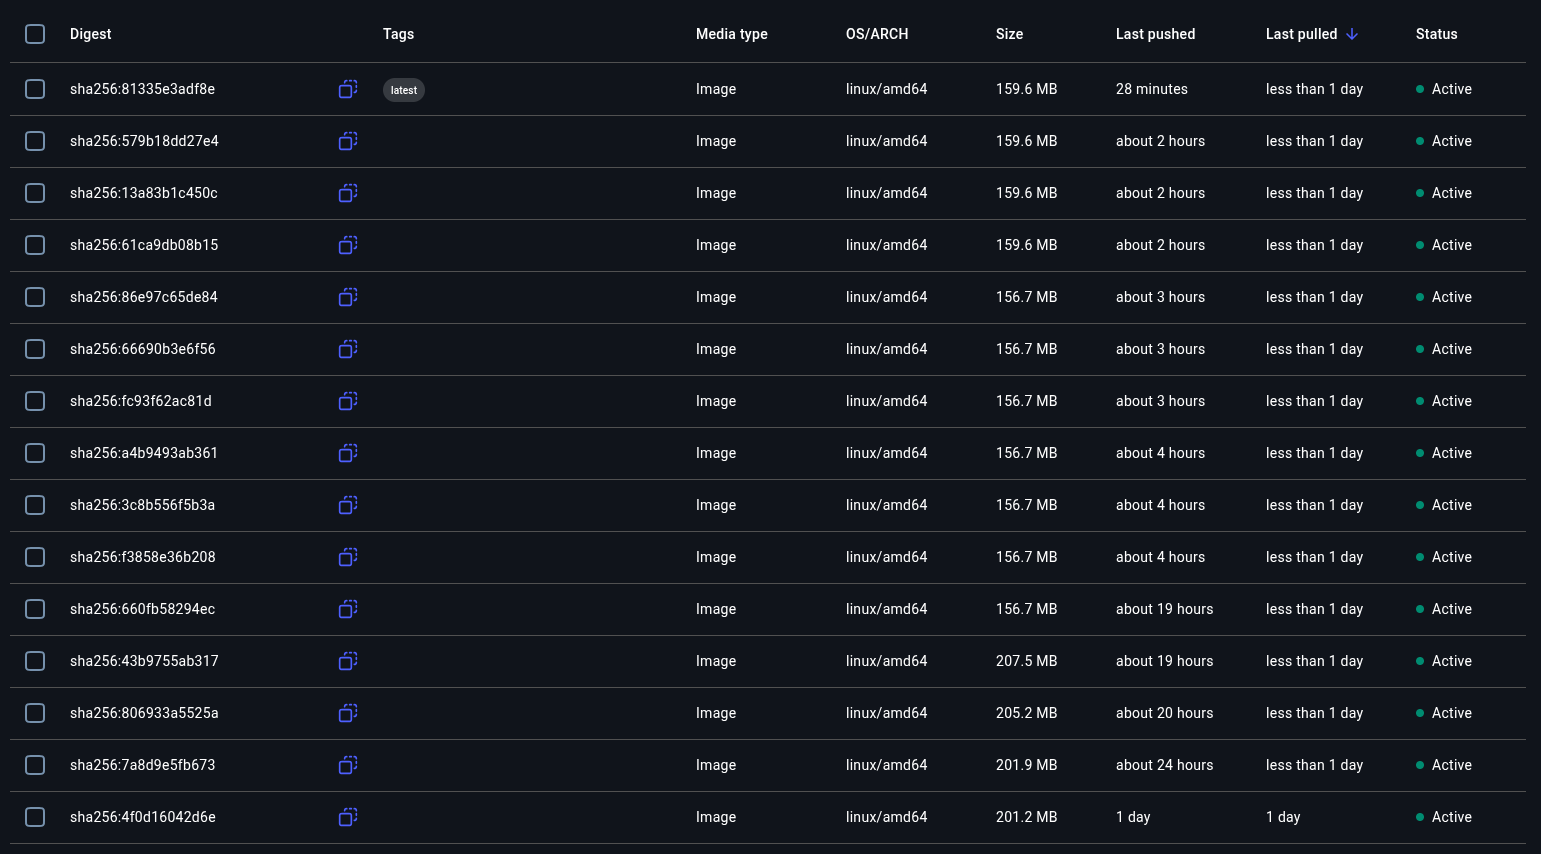
\includegraphics[width=1.0\textwidth]{images/docker-hub-commits.png}
    \caption{Published Docker Images hosted at Docker Hub natively tracking commits.}
\end{figure}

\newpage

\section{Pipeline Execution and Observability}

The following screenshots outline the successful execution of the Jenkins architecture across iterative DevOps branches.

\begin{figure}[H]
    \centering
    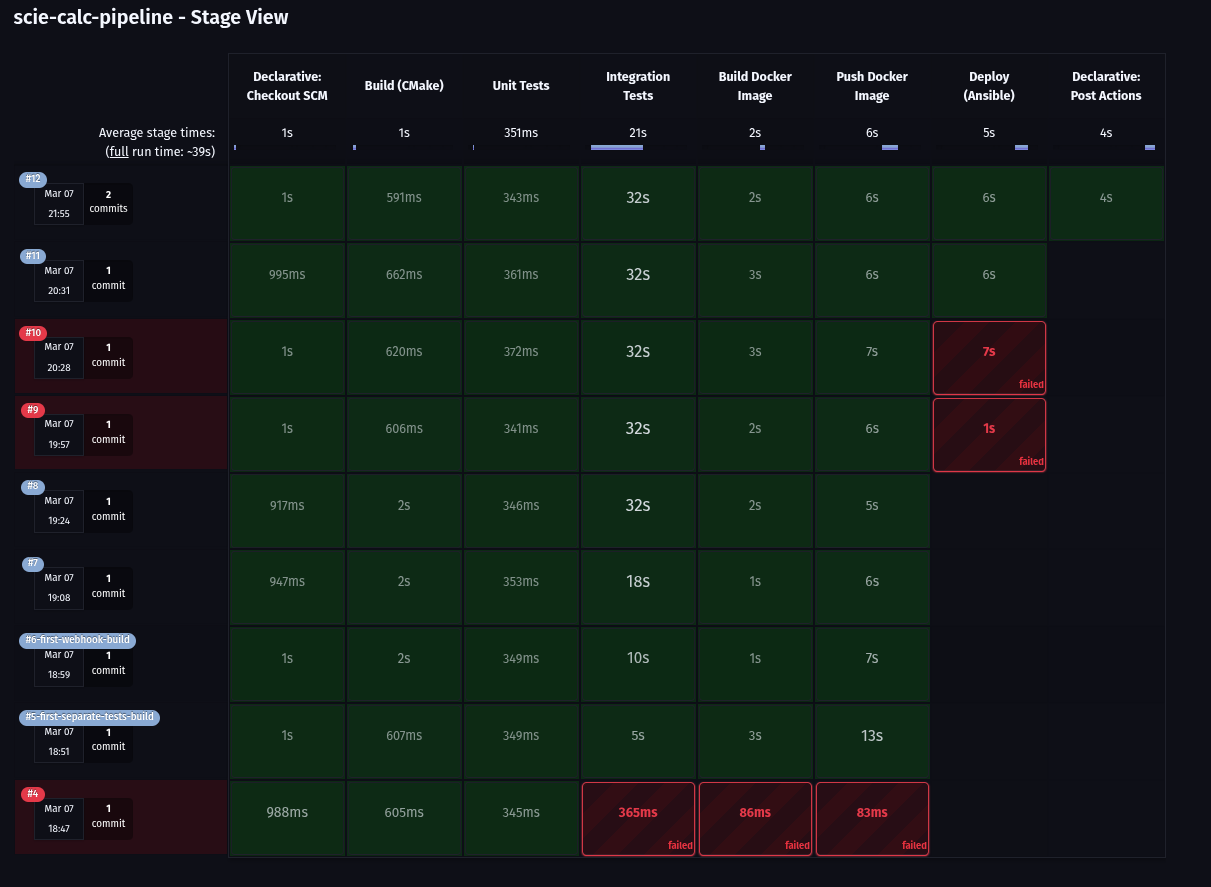
\includegraphics[width=0.9\textwidth]{images/stage_view.png}
    \caption{Jenkins Stage View highlighting the explicit pipeline steps and their execution times.}
\end{figure}

\begin{figure}[H]
    \centering
    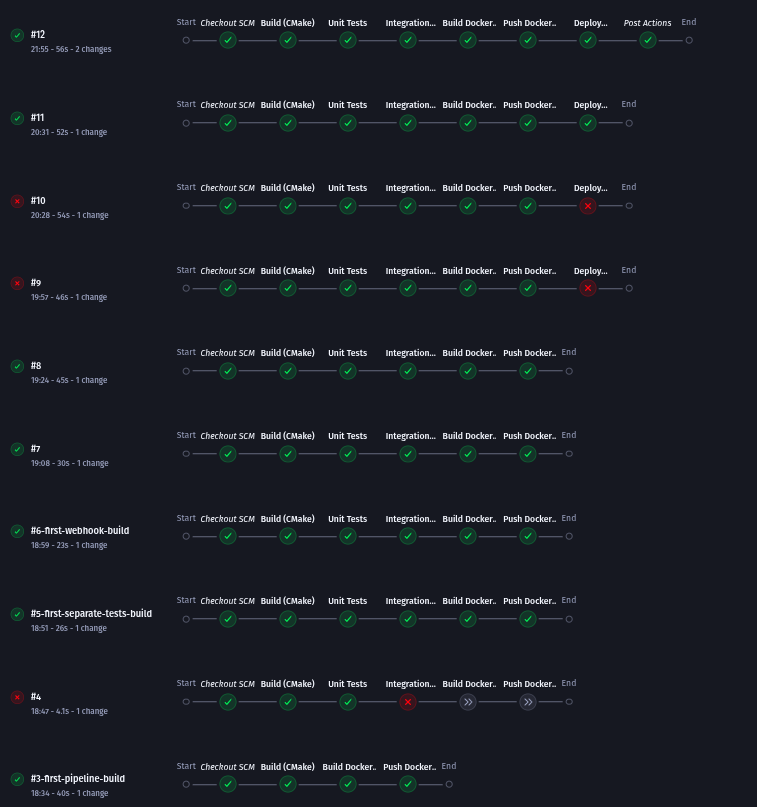
\includegraphics[width=0.9\textwidth]{images/jenkins_pipeline.png}
    \caption{Jenkins Pipeline Execution completing safely with all stages green. This proves the codebase successfully compiled, passed all assertions, packaged into Docker, and deployed via Ansible sequentially without error.}
\end{figure}

\begin{figure}[H]
    \centering
    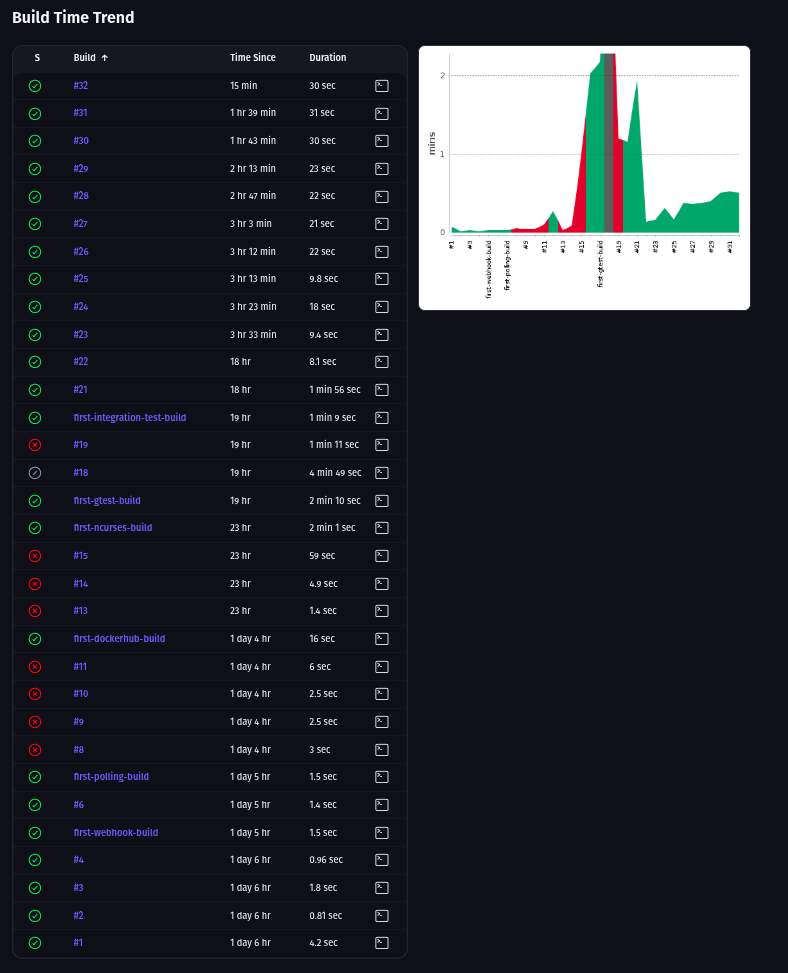
\includegraphics[width=0.9\textwidth]{images/jenkins_build_trend.png}
    \caption{Build Time Trend and Execution History in Jenkins tracking historical failure rates during initial test implementations natively resolving to rapid successful durations. Notice the sharp decline in build duration; this represents the implementation of Docker BuildKit caching mechanisms dropping the entire CI/CD pipeline execution length down to under 30 seconds.}
\end{figure}

\begin{figure}[H]
    \centering
    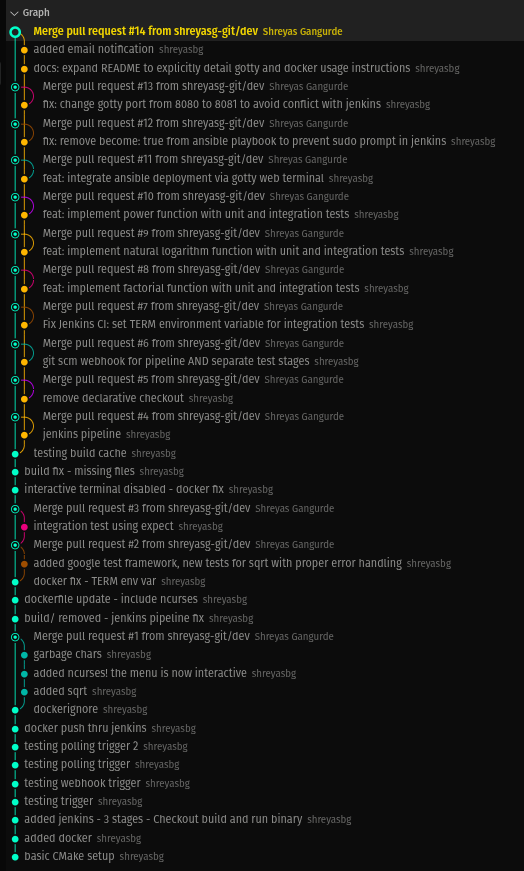
\includegraphics[width=0.9\textwidth]{images/git_branch_visualization.png}
    \caption{Git Branch Visualization tracking chronological commits mapping feature additions (Factorial, Natural Log, Power functions) and the incremental building of the CI/CD pipeline infrastructure leading to the remote deployment.}
\end{figure}

\newpage

\section{Test Results and Observations}

The pipeline executes dual-layer testing protocols ensuring absolute reliability before touching a production deployment.

\subsection{Unit Test Results (Google Test)}
Google Test successfully evaluated the `src/calculator.cpp` logic. 

\textbf{Observations:}
\begin{itemize}
    \item \textbf{Positive Validations:} The engine accurately calculates standard expected values (e.g., $4^2 = 16$, $\sqrt{16} = 4$, and $\ln(e) = 1$).
    
    \item \textbf{Negative/Boundary Validations:} The codebase correctly throws explicit exceptions \texttt{std::invalid\_argument}, preventing systematic crashes. The tests successfully proved that calculating the square root of a negative number, the factorial of a negative integer, or the natural logarithm of $0$ are all safely caught and handled by our model structure rather than crashing the interface.
\end{itemize}

\subsection{Integration Test Results (Expect Automation)}
The Expect shell scripting natively simulated end-user keystrokes launching the compiled binary.

\textbf{Observations:}
\begin{itemize}
    \item Navigational bounds were tested (i.e., pressing "Up/Down" to cycle through Square Root, Factorial, Natural Log, and Power menus).
    \item Validated that when a user types a mathematically illegal argument directly into the user interface, the \texttt{ncurses} terminal properly halts, alerts the user to "Press any key to continue", and safely routes the user back to the Main Menu rather than exiting the process.
\end{itemize}


\section{Application Showcase}
Below denotes the application serving gracefully over the target browser window utilizing Web Sockets (Gotty). The user interface is driven effectively utilizing C++ NCurses parsing arrow-key iterations accurately.

\begin{figure}[H]
    \centering
    
\includegraphics[width=0.8\textwidth]{images/menu.png}
    \caption{Application Main Menu (Ncurses interface rendered via WebTTY).}
\end{figure}

\begin{figure}[H]
    \centering
    
\includegraphics[width=0.8\textwidth]{images/square_root.png}
    \caption{Executing a Square Root calculation spanning valid positive numbers and floating points.}
\end{figure}

\begin{figure}[H]
    \centering
    
\includegraphics[width=0.8\textwidth]{images/factorial.png}
    \caption{Executing a Factorial calculation over the deployment infrastructure.}
\end{figure}

\begin{figure}[H]
    \centering
    
\includegraphics[width=0.8\textwidth]{images/natural_log.png}
    \caption{Executing a Natural Logarithm evaluation seamlessly via the Web Terminal.}
\end{figure}

\begin{figure}[H]
    \centering
    
\includegraphics[width=0.8\textwidth]{images/exponent.png}
    \caption{Executing an Exponential Power calculation natively over the live Gotty feed.}
\end{figure}


\section{Links and References}
\begin{itemize}
    \item \textbf{GitHub Source Code Repository:}
    \newline\url{https://github.com/shreyasg-git/spe-mini-scie-calc.git}
    \item \textbf{Docker Hub Container Registry:} \url{https://hub.docker.com/r/shreyasg28/sci-calc}
\end{itemize}


\end{document}
